\documentclass[11pt]{article}
\usepackage[margin=0.75in]{geometry}
\usepackage{booktabs}
\usepackage{caption}
\usepackage{float}
\usepackage{graphicx}
\usepackage{adjustbox}

\title{BigRAG Cinema -- Tentative Benchmark Results}
\author{Robby Moseley}
\date{\today}

\begin{document}
\maketitle

\section*{Overview}
Benchmark results from 5 Amazon Reviews 2023 categories totaling approximately 20 million records. Four hybrid query execution strategies benchmarked at 5 data fractions (10\%--100\%) using Apache Spark in local mode on a 16-CPU / 64GB SLURM node.

\begin{table}[ht]
\centering
\begin{tabular}{lrrr}
\hline
Dataset & Total Rows & Queries & Repetitions \\
\hline
All Beauty & 693,548 & 50 & 3 \\
Amazon Fashion & 2,473,302 & 50 & 2 \\
Appliances & 2,103,927 & 50 & 2 \\
Arts \& Crafts & 8,859,715 & 30 & 1 \\
Baby Products & 5,962,394 & 30 & 1 \\
\hline
\textbf{Total} & \textbf{20,092,886} & & \\
\hline
\end{tabular}
\caption{Benchmark dataset summary from the Amazon Reviews 2023 corpus.}
\label{tab:datasets}
\end{table}

\begin{table*}[ht]
\centering
\small
\adjustbox{max width=\textwidth}{%
\begin{tabular}{lrrrrr}
\hline
Strategy & All Beauty (694K) & Amazon Fashion (2.5M) & Appliances (2.1M) & Arts \& Crafts (8.9M) & Baby Products (6.0M) \\
\hline
\multicolumn{6}{l}{\textit{Median Latency (ms)}} \\
\hline
Filter-First & \textbf{1,245} & 4,652 & 3,728 & 17,126 & 13,047 \\
Vector-First & \textbf{13,435} & 48,002 & 41,046 & 172,191 & 119,110 \\
Hybrid Parallel & \textbf{13,440} & 47,923 & 40,827 & 171,459 & 115,428 \\
Adaptive & \textbf{1,289} & 4,508 & 3,735 & 16,619 & 12,489 \\
\hline
\multicolumn{6}{l}{\textit{P99 Latency (ms)}} \\
\hline
Filter-First & \textbf{9,352} & 33,574 & 27,069 & 111,673 & 70,001 \\
Vector-First & \textbf{13,556} & 48,210 & 41,323 & 172,827 & 121,202 \\
Hybrid Parallel & \textbf{13,580} & 48,194 & 41,062 & 172,547 & 116,679 \\
Adaptive & \textbf{13,553} & 48,342 & 41,127 & 171,667 & 118,556 \\
\hline
\multicolumn{6}{l}{\textit{Mean Throughput (qps)}} \\
\hline
Filter-First & \textbf{0.69} & 0.19 & 0.23 & 0.05 & 0.07 \\
Vector-First & \textbf{0.07} & 0.02 & 0.02 & 0.01 & 0.01 \\
Hybrid Parallel & \textbf{0.07} & 0.02 & 0.02 & 0.01 & 0.01 \\
Adaptive & \textbf{0.66} & 0.19 & 0.22 & 0.05 & 0.07 \\
\hline
\end{tabular}}
\caption{Cross-dataset strategy comparison at full data scale. Bold indicates best strategy per dataset per metric.}
\label{tab:cross-dataset}
\end{table*}

\begin{table*}[ht]
\centering
\small
\adjustbox{max width=\textwidth}{%
\begin{tabular}{lrrrrrrrrrr}
\hline
Strategy & \multicolumn{2}{c}{All Beauty} & \multicolumn{2}{c}{Amazon Fashion} & \multicolumn{2}{c}{Appliances} & \multicolumn{2}{c}{Arts \& Crafts} & \multicolumn{2}{c}{Baby Products} \\
 & 10\% (ms) & Factor & 10\% (ms) & Factor & 10\% (ms) & Factor & 10\% (ms) & Factor & 10\% (ms) & Factor \\
\hline
Filter-First & 173 & 7.2$\times$ & 484 & 9.6$\times$ & 423 & 8.8$\times$ & 1,595 & 10.7$\times$ & 1,193 & 10.9$\times$ \\
Vector-First & 1,380 & 9.7$\times$ & 4,820 & 10.0$\times$ & 4,133 & 9.9$\times$ & 17,031 & 10.1$\times$ & 11,601 & 10.3$\times$ \\
Hybrid Parallel & 1,407 & 9.5$\times$ & 4,839 & 9.9$\times$ & 4,149 & 9.8$\times$ & 17,134 & 10.0$\times$ & 11,595 & 10.0$\times$ \\
Adaptive & 199 & 6.5$\times$ & 508 & 8.9$\times$ & 448 & 8.3$\times$ & 1,645 & 10.1$\times$ & 1,172 & 10.7$\times$ \\
\hline
\end{tabular}}
\caption{Scalability analysis: median latency at 10\% data fraction and growth factor to full scale (100\%). Lower factor = better scalability.}
\label{tab:scalability}
\end{table*}

\begin{table*}[ht]
\centering
\small
\adjustbox{max width=\textwidth}{%
\begin{tabular}{lrrrrr}
\hline
Comparison & All Beauty & Amazon Fashion & Appliances & Arts \& Crafts & Baby Products \\
\hline
vs. Vector-First & 10.8$\times$ & 10.3$\times$ & 11.0$\times$ & 10.1$\times$ & 9.1$\times$ \\
vs. Hybrid Parallel & 10.8$\times$ & 10.3$\times$ & 11.0$\times$ & 10.0$\times$ & 8.8$\times$ \\
vs. Adaptive & 1.0$\times$ & 1.0$\times$ & 1.0$\times$ & 1.0$\times$ & 1.0$\times$ \\
\hline
\end{tabular}}
\caption{Speedup of Filter-First over other strategies (median latency ratio at full scale). Higher = Filter-First is faster by that factor.}
\label{tab:speedup}
\end{table*}

\begin{table*}[ht]
\centering
\small
\adjustbox{max width=\textwidth}{%
\begin{tabular}{llllll}
\hline
Metric & All Beauty & Amazon Fashion & Appliances & Arts \& Crafts & Baby Products \\
\hline
Median Latency & Filter-First & Adaptive & Filter-First & Adaptive & Adaptive \\
P99 Latency & Filter-First & Filter-First & Filter-First & Filter-First & Filter-First \\
Mean Throughput & Filter-First & Adaptive & Filter-First & Adaptive & Adaptive \\
Latency Variance & Vector-First & Vector-First & Hybrid Parallel & Vector-First & Hybrid Parallel \\
\hline
\textbf{Total Wins} & Filter-First (3/4) & Adaptive (2/4) & Filter-First (3/4) & Adaptive (2/4) & Adaptive (2/4) \\
\hline
\end{tabular}}
\caption{Best-performing strategy per dataset at full scale. Latency Variance measured as P99/P50 ratio (lower = more consistent).}
\label{tab:winners}
\end{table*}

\begin{table}[ht]
\centering
\small
\begin{tabular}{llrrrrr}
\hline
Strategy & Fraction & P50 & P95 & P99 & Min & Max \\
\hline
Filter-First & 10\% & 1,595 & 8,215 & 11,160 & 1,574 & 11,844 \\
 & 25\% & 3,924 & 20,200 & 27,079 & 3,844 & 28,642 \\
 & 50\% & 8,086 & 41,292 & 55,473 & 7,616 & 58,660 \\
 & 75\% & 12,740 & 62,364 & 83,605 & 11,446 & 88,445 \\
 & 100\% & 17,126 & 82,351 & 111,673 & 15,430 & 118,225 \\
\hline
Vector-First & 10\% & 17,031 & 17,115 & 17,126 & 16,954 & 17,129 \\
 & 25\% & 42,602 & 42,783 & 42,919 & 42,419 & 42,964 \\
 & 50\% & 85,572 & 85,860 & 85,908 & 85,329 & 85,925 \\
 & 75\% & 128,581 & 128,956 & 129,215 & 128,127 & 129,296 \\
 & 100\% & 172,191 & 172,741 & 172,827 & 171,458 & 172,861 \\
\hline
Hybrid Parallel & 10\% & 17,134 & 17,245 & 17,290 & 17,014 & 17,306 \\
 & 25\% & 42,625 & 42,925 & 42,946 & 42,477 & 42,950 \\
 & 50\% & 85,458 & 85,823 & 85,907 & 84,877 & 85,932 \\
 & 75\% & 127,855 & 128,236 & 128,306 & 127,251 & 128,325 \\
 & 100\% & 171,459 & 172,195 & 172,547 & 170,553 & 172,680 \\
\hline
Adaptive & 10\% & 1,645 & 17,332 & 17,414 & 1,598 & 17,425 \\
 & 25\% & 4,029 & 43,270 & 43,504 & 3,863 & 43,546 \\
 & 50\% & 8,341 & 85,409 & 85,607 & 7,680 & 85,660 \\
 & 75\% & 12,819 & 128,097 & 128,235 & 11,521 & 128,285 \\
 & 100\% & 16,619 & 171,282 & 171,667 & 15,254 & 171,730 \\
\hline
\end{tabular}
\caption{Latency percentile breakdown (ms) -- Arts \& Crafts.}
\label{tab:percentiles-arts_crafts_and_sewing}
\end{table}

\begin{table}[ht]
\centering
\small
\begin{tabular}{llrrrr}
\hline
Strategy & Fraction & Median Lat. (ms) & P95 Lat. (ms) & Throughput (qps) & Results \\
\hline
Filter-First & 10\% & 1,595 & 8,215 & 0.54 & 3.3 \\
 & 25\% & 3,924 & 20,200 & 0.22 & 3.3 \\
 & 50\% & 8,086 & 41,292 & 0.11 & 3.3 \\
 & 75\% & 12,740 & 62,364 & 0.07 & 3.3 \\
 & 100\% & 17,126 & 82,351 & 0.05 & 3.3 \\
\hline
Vector-First & 10\% & 17,031 & 17,115 & 0.06 & 1.9 \\
 & 25\% & 42,602 & 42,783 & 0.02 & 1.9 \\
 & 50\% & 85,572 & 85,860 & 0.01 & 1.8 \\
 & 75\% & 128,581 & 128,956 & 0.01 & 1.8 \\
 & 100\% & 172,191 & 172,741 & 0.01 & 1.7 \\
\hline
Hybrid Parallel & 10\% & 17,134 & 17,245 & 0.06 & 3.3 \\
 & 25\% & 42,625 & 42,925 & 0.02 & 3.3 \\
 & 50\% & 85,458 & 85,823 & 0.01 & 3.3 \\
 & 75\% & 127,855 & 128,236 & 0.01 & 3.3 \\
 & 100\% & 171,459 & 172,195 & 0.01 & 3.3 \\
\hline
Adaptive & 10\% & 1,645 & 17,332 & 0.51 & 3.3 \\
 & 25\% & 4,029 & 43,270 & 0.21 & 3.3 \\
 & 50\% & 8,341 & 85,409 & 0.10 & 3.3 \\
 & 75\% & 12,819 & 128,097 & 0.07 & 3.3 \\
 & 100\% & 16,619 & 171,282 & 0.05 & 3.3 \\
\hline
\end{tabular}
\caption{Detailed benchmark results -- Arts \& Crafts.}
\label{tab:detail-arts_crafts_and_sewing}
\end{table}

%% ---------- Recall & Shuffle Tables ----------
\IfFileExists{table_recall.tex}{\begin{table*}[ht]
\centering
\small
\begin{tabular}{lrrr}
\hline
Strategy & All Beauty & Digital Music & Mean \\
\hline
Filter-First & \textbf{1.0000} & \textbf{1.0000} & \textbf{1.0000} \\
Vector-First & 0.8100 & 0.9700 & 0.8900 \\
Hybrid Parallel & \textbf{1.0000} & \textbf{1.0000} & \textbf{1.0000} \\
Adaptive & \textbf{1.0000} & \textbf{1.0000} & \textbf{1.0000} \\
\hline
\multicolumn{4}{l}{\textit{By Selectivity Bucket (first dataset)}} \\
\hline
Filter-First & Low: 1.0 & Med: 1.0 & High: 1.0 \\
Vector-First & Low: 1.0 & Med: 1.0 & High: 0.3667 \\
Hybrid Parallel & Low: 1.0 & Med: 1.0 & High: 1.0 \\
Adaptive & Low: 1.0 & Med: 1.0 & High: 1.0 \\
\hline
\end{tabular}
\caption{Recall@10 per strategy. Filter-First serves as ground truth (recall=1.0). Bold indicates perfect recall.}
\label{tab:recall-at-10}
\end{table*}}{}
\IfFileExists{table_shuffle_cost.tex}{\input{table_shuffle_cost.tex}}{}

%% ---------- Figures ----------
\clearpage
\section*{Figures}

\begin{figure}[H]
\centering

\includegraphics[width=\textwidth]{../figures/scaling_curves.png}
\caption{Latency scaling curves across data fractions.}
\end{figure}

\begin{figure}[H]
\centering

\includegraphics[width=\textwidth]{../figures/throughput_bars.png}
\caption{Throughput comparison by strategy.}
\end{figure}

\begin{figure}[H]
\centering

\includegraphics[width=\textwidth]{../figures/latency_boxplots.png}
\caption{Latency distribution boxplots.}
\end{figure}

\begin{figure}[H]
\centering

\includegraphics[width=\textwidth]{../figures/latency_heatmap.png}
\caption{Latency heatmap across strategies and fractions.}
\end{figure}

\begin{figure}[H]
\centering

\includegraphics[width=\textwidth]{../figures/percentile_bars.png}
\caption{Latency percentile bars (P50, P95, P99).}
\end{figure}

\begin{figure}[H]
\centering

\includegraphics[width=\textwidth]{../figures/latency_cdf.png}
\caption{Latency CDF across strategies.}
\end{figure}

\begin{figure}[H]
\centering
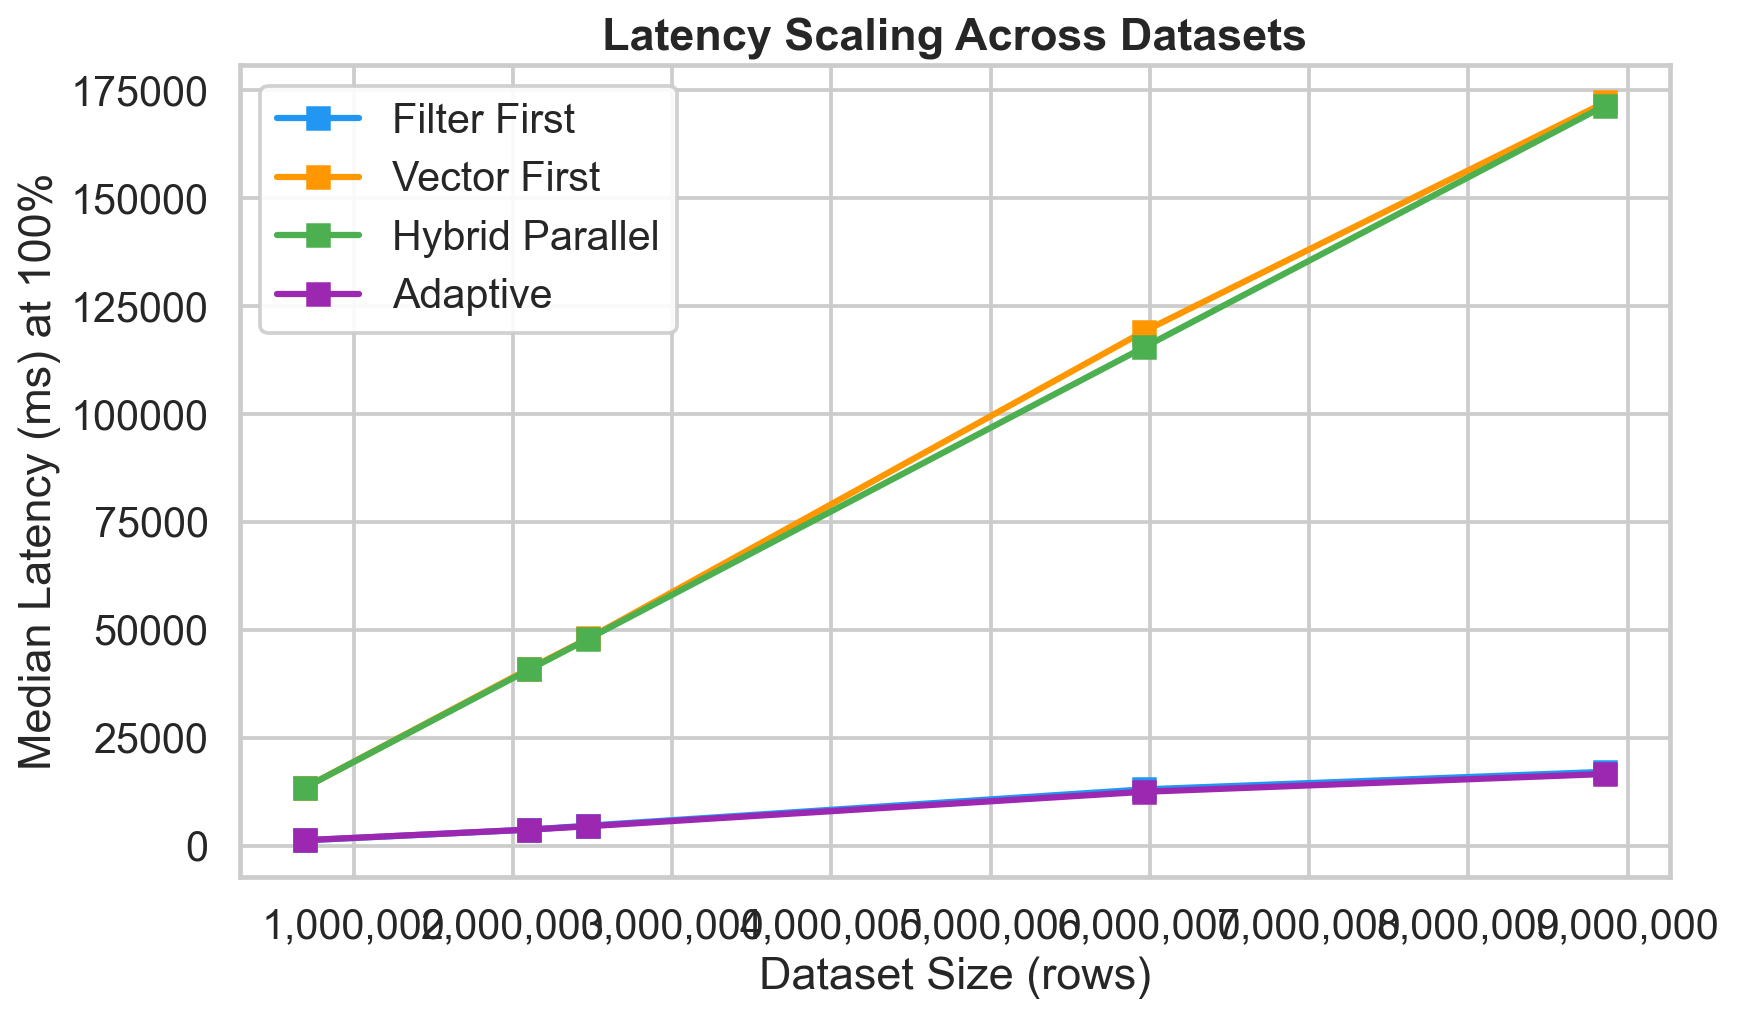
\includegraphics[width=\textwidth]{../figures/comparison/cross_dataset_scaling.png}
\caption{Cross-dataset latency scaling comparison.}
\end{figure}

\begin{figure}[H]
\centering
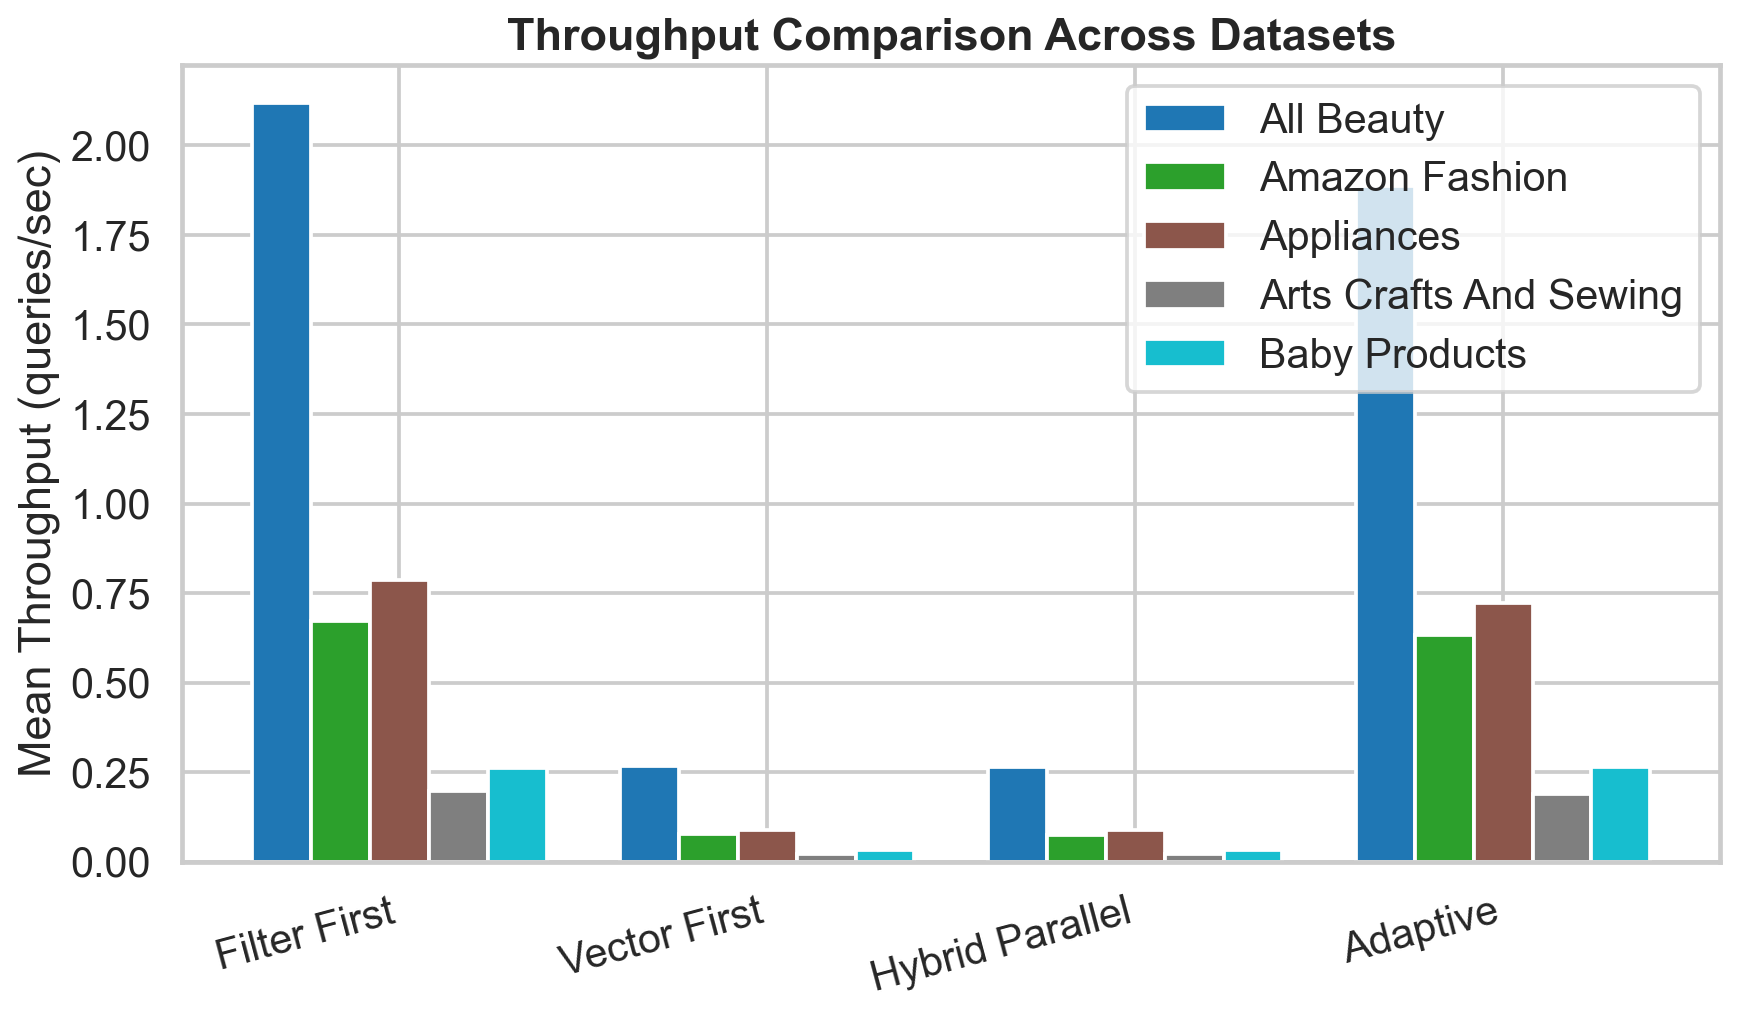
\includegraphics[width=\textwidth]{../figures/comparison/cross_dataset_throughput.png}
\caption{Cross-dataset throughput comparison.}
\end{figure}

\end{document}
